\documentclass[a4paper]{article}
\usepackage{graphicx}
\usepackage{hyperref}
\usepackage[inner=0.5cm,outer=0.5cm]{geometry}
\usepackage{mathtools}
\begin{document}

\title{Least Common Subsequence}
\author{Dmitri Kovalenko}

\maketitle
\section{Analysis}
\begin{align*}
    &  n = \text{problem size}\\
    &  p = \text{processors amont}\\
    &  s = \text{chunk stride} = \alpha  p\\
    &  l = \text{chunk length} = n/s\\
    &  T_{\text{comp}} = (2s-1) \cdot {\frac{n^2}{s^2}} = O(\frac{n^2}{p})\\
    &  T_{\text{comm}} = (2s-1) \cdot l = O(n)\\
    &  T_{\text{sync}} = 2s-1 = O(p)
\end{align*}

\section{Results}
    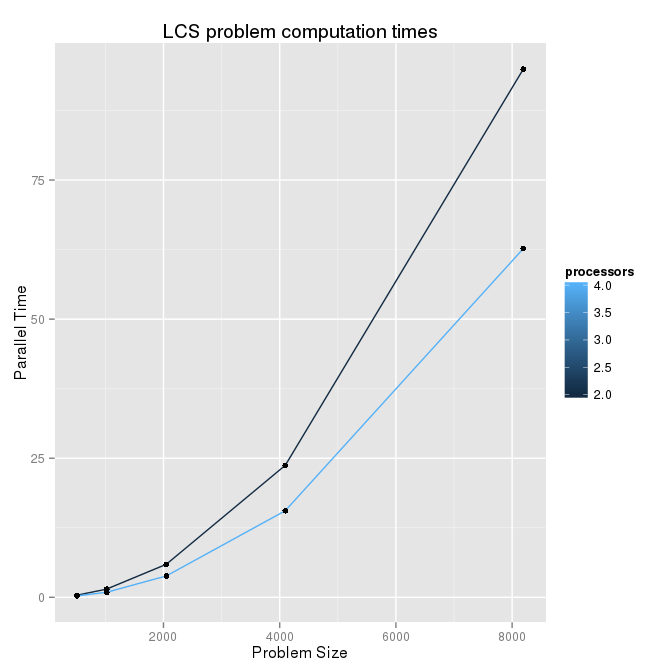
\includegraphics[width=0.45\textwidth]{lcs}
    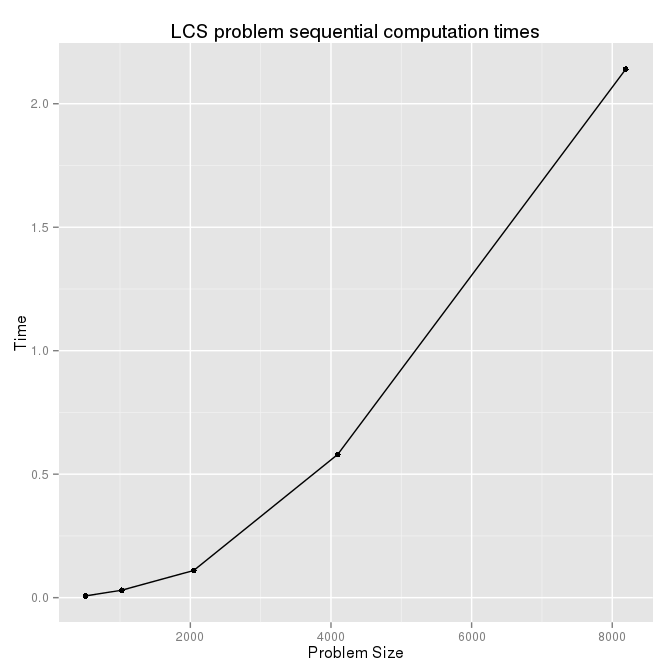
\includegraphics[width=0.45\textwidth]{lcs-seq}

\section{Links}
\begin{enumerate}
    \item Peter Krusche and Alexander Tiskin Efficient Longest Common Subsequence
            Computation using Bulk-Synchronous Parallelism 2006 \url{http://www.dcs.warwick.ac.uk/~tiskin/pub/2006/iccsa.pdf}
  \item  A. Tiskin Advanced Topics in Algorithms \url{http://www2.warwick.ac.uk/fac/sci/dcs/teaching/material/cs341/ata_handout1.pdf}
  \item Peter Krusche and Alexander Tiskin Efficient Parallel String Comparison 2007 \url{http://www.booksonline.iospress.nl/Content/View.aspx?piid=8388}
\end{enumerate}

\end{document}

